% Two-point propagator flow without cutoff derivative

\documentclass[tikz]{standalone}

\usetikzlibrary{patterns,decorations.markings}

\tikzset{
  dressed/.style={fill=white,postaction={pattern=north east lines}},
  momentum/.style={->,semithick,yshift=5pt,shorten >=5pt,shorten <=5pt},
  loop/.style 2 args={thick,decoration={markings,mark=at position {#1} with {\arrow{>},\node[anchor=\pgfdecoratedangle-90,font=\footnotesize] {$p_{#2}$};}},postaction={decorate}},
  label/.style={thin,gray,shorten <=-1ex}
}

\def\lrad{1}
\def\mrad{0.175*\lrad}
\def\srad{0.15*\lrad}

\begin{document}

% Diagram 1
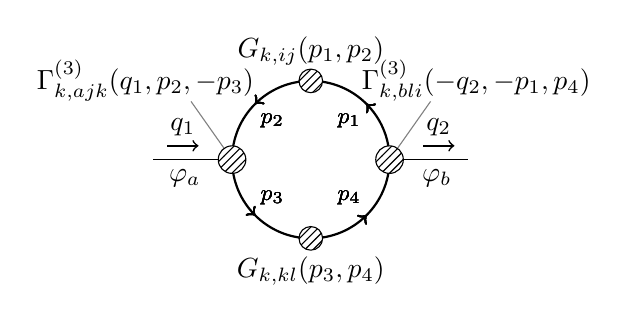
\begin{tikzpicture}
  % Loop
  \draw[loop/.list={{0.125}{1},{0.125*3}{2},{0.125*5}{3},{0.125*7}{4}}] (0,0) circle (\lrad);
  \draw[dressed] (0,\lrad) circle (\srad) node[above=2pt] {$G_{k,ij}(p_1,p_2)$};
  \draw[dressed] (0,-\lrad) circle (\srad) node[below=3pt] {$G_{k,kl}(p_3,p_4)$};

  % External lines
  \draw (-2*\lrad,0) coordinate (xl) -- (-\lrad,0) node[pos=0.4,below] {$\varphi_a$};
  \draw[momentum] (-2*\lrad,0) -- (-1.25*\lrad,0) node[midway,above] {$q_1$};
  \draw (\lrad,0) -- (2*\lrad,0) coordinate (xr) node[pos=0.6,below] {$\varphi_b$};
  \draw[momentum] (1.25*\lrad,0) -- (2*\lrad,0) node[midway,above] {$q_2$};

  % Vertices
  \node at (-2.1*\lrad,\lrad) (Gkajk) {$\Gamma_{k,ajk}^{(3)}(q_1,p_2,-p_3)$};
  \draw[label] (Gkajk.-30) -- (-\lrad,0);
  \draw[dressed] (-\lrad,0) circle (\mrad);
  \node at (2.1*\lrad,\lrad) (Gkbli) {$\Gamma_{k,bli}^{(3)}(-q_2,-p_1,p_4)$};
  \draw[label] (Gkbli.-150) -- (\lrad,0);
  \draw[dressed] (\lrad,0) circle (\mrad);
\end{tikzpicture}

% Diagram 2
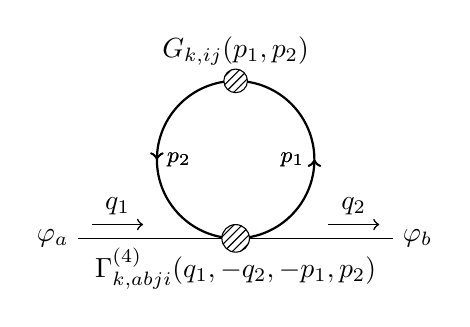
\begin{tikzpicture}
  % Loop
  \draw[loop/.list={{0}{1},{0.125*4}{2}}] (0,0) circle (\lrad);
  \draw[dressed] (0,\lrad,0) circle (\srad) node[above=2pt] {$G_{k,ij}(p_1,p_2)$};

  % External lines
  \draw (-2*\lrad,-\lrad) node[left] {$\varphi_a$} -- (2*\lrad,-\lrad) node[right] {$\varphi_b$};
  \draw[momentum] (-2*\lrad,-\lrad) -- (-\lrad,-\lrad) node[midway,above] {$q_1$};
  \draw[momentum] (\lrad,-\lrad) -- (2*\lrad,-\lrad) node[midway,above] {$q_2$};

  % Vertices
  \draw[dressed] (0,-\lrad) circle (\mrad) node[below] {$\Gamma_{k,abji}^{(4)}(q_1,-q_2,-p_1,p_2)$};
\end{tikzpicture}

\end{document}